% ============================================================================
% part6/appEndix E --- Relational Formulation of chi Dynamics
% From former part6/appEndix E of Cosmochrony v1.13beta1, streamlined
% ============================================================================
\clearpage

\section{Relational Formulation of
\texorpdfstring{$\chi$}{χ} Dynamics}
\label{app:relational_formulation}

This part6/appEndix develops a fully relational and explicitly non-geometric
formulation of $\chi$ dynamics.
It clarifies how particle-like properties, topological stability, and
quantum correlations arise from the intrinsic relational structure
of~$\chi$, prior to the emergence of geometry.

The relational formulation does not assume a background spacetime or
metric, spatial localization, a tensorial or spinorial fundamental
ontology, or an underlying Hilbert space structure.
Particle-like excitations are identified with internally stable
relational configurations whose apparent properties---mass, charge, spin,
statistics---emerge from topological and organizational features once a
projectable regime applies.

% ----------------------------------------------------------------------------
% E.1 --- Relational Configurations of chi
% From former E.1, condensed
% ----------------------------------------------------------------------------
\subsection{Relational Configurations of
\texorpdfstring{$\chi$}{χ}}
\label{subsec:relational-configurations-of-chi}

A relational configuration of~$\chi$ is defined by its internal pattern
of mutual relaxation constraints, without coordinates, distances, or
background geometry
(Section~\ref{subsec:definition-of-the-chi-field}).
Physical states correspond to equivalence classes under
relaxation-preserving transformations.
Configurations do not generally factorize into independent subsystems;
this structural non-factorization underlies nonlocal correlations
(Section~\ref{subsec:non-factorization-entanglement}).
Only under conditions of approximate homogeneity and stable relaxation
does a relational configuration admit an effective geometric projection,
via a many-to-one, inherently approximate mapping.

% ----------------------------------------------------------------------------
% E.2 --- Non-Factorization and Entanglement
% From former E.2, condensed
% ----------------------------------------------------------------------------
\subsection{Non-Factorization and Entanglement}
\label{subsec:non-factorization-entanglement}

Factorization---decomposition preserving internal relaxation structure
while isolating disjoint subsets of relations---is not fundamental but
emerges only in restricted regimes.
Quantum entanglement arises as a direct manifestation of persistent
non-factorization: when a non-factorizable relational configuration
admits an effective projection onto spatially separated degrees of
freedom, its components remain relationally inseparable.

\paragraph{Projection-induced non-factorization.}
Because the projection
$\Pi:\mathcal{C}_\chi \rightarrow \mathcal{C}_{\mathrm{eff}}$ is
generically non-injective, a single effective configuration~$y$
corresponds to an equivalence class
\begin{equation}
  \Pi^{-1}(y) \subset \mathcal{C}_\chi .
\end{equation}
Entanglement arises when this fiber contains globally constrained
configurations that do not admit decomposition into independent
substructures compatible with the effective subsystem decomposition.
No conditioning on underlying relational degrees of freedom can restore
a product structure for joint outcome statistics.

\paragraph{Compression and limits of entanglement.}
Entanglement persists only in an intermediate regime where projection
preserves sufficient global relational structure to prevent
factorization, while still allowing stable decomposition into effective
subsystems.
If projection is effectively injective, fibers collapse to single
elements and factorization is recovered; if excessively
coarse-grained, relational constraints are erased and descriptions
become fully factorized.

% ----------------------------------------------------------------------------
% E.3 --- Locality, Causality, and the Role of the Bound c
% From former E.3, preserved (already minimal)
% ----------------------------------------------------------------------------
\subsection{Locality, Causality, and the Role of the Bound
\texorpdfstring{$c$}{c}}
\label{subsec:locality-causality-and-the-role-of-the-bound-c}

Correlations between configurations of~$\chi$ may extend across
arbitrarily large effective distances once a geometric description
applies.
However, all modifications of relational configurations are constrained
by a universal kinematic bound~$c$.

\input{part6/appE/sec-distance-chieff}
% ----------------------------------------------------------------------------
% E.5 --- Emergent Coordinates via Manifold Reconstruction
% From former E.7, condensed
% ----------------------------------------------------------------------------
\subsection{Emergent Coordinates via Manifold Reconstruction}
\label{subsec:emergent-coordinates}

When the relational distance matrix $D=\{d_{ij}\}$ admits a
low-dimensional embedding, coordinates can be reconstructed using
multidimensional scaling.
The centered Gram matrix is
\begin{equation}
  G_{ij} = -\tfrac{1}{2}\Big(
    d_{ij}^2 - d_{i\cdot}^2
    - d_{\cdot j}^2 + d_{\cdot\cdot}^2\Big),
  \label{eq:gram-matrix}
\end{equation}
yielding eigenpairs $(\lambda_k, v_k)$ and an embedding
\begin{equation}
  x_i^{(a)} = \sqrt{\lambda_a}\,(v_a)_i,
  \quad a=1,\dots,d.
  \label{eq:mds-embedding}
\end{equation}
The intrinsic dimension~$d$ is selected by the eigenvalue gap:
\begin{equation}
  \Delta\lambda_{d+1} > \eta\,\lambda_1,
  \label{eq:eigen-gap-criterion}
\end{equation}
with $\eta \sim 0.1$.
For smooth large-scale configurations, a stable $d=4$ embedding is
expected.

\begin{figure}[t]
  \centering
  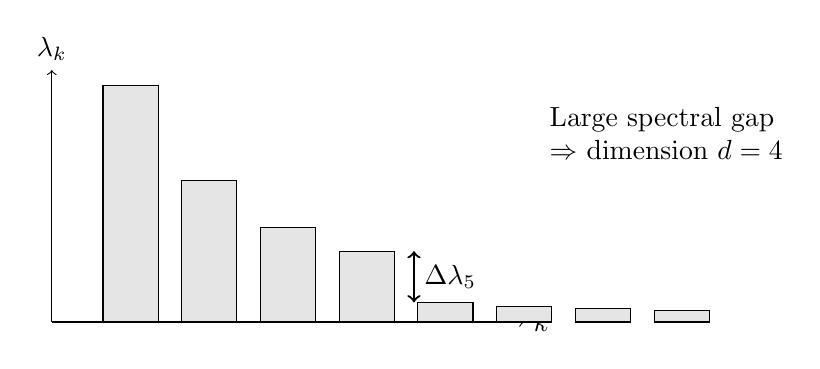
\begin{tikzpicture}[scale=1.0]
    \draw[->] (0,0) -- (6,0) node[right]{$k$};
    \draw[->] (0,0) -- (0,3.2) node[above]{$\lambda_k$};
    \foreach \k/\h in
      {1/3.0,2/1.8,3/1.2,4/0.9,5/0.25,6/0.20,
       7/0.17,8/0.15} {
      \draw[fill=black!10]
        (\k-0.35,0) rectangle (\k+0.35,\h);
    }
    \draw[<->, thick]
      (4.6,0.9) -- (4.6,0.25)
      node[midway,right]{$\Delta\lambda_5$};
    \node[align=left, anchor=west] at (6.2,2.4)
      {Large spectral gap\\
       $\Rightarrow$ dimension $d=4$};
  \end{tikzpicture}
  \caption{Schematic eigenvalue spectrum for intrinsic
    dimension selection.
    A clear gap after four modes indicates a robust $d=4$
    projectable regime.}
  \label{fig:eigenvalue-gap}
\end{figure}

Failure of the reconstruction (non-local connectivity or no clear
spectral gap) signals a transition to a pre-geometric regime where a
smooth manifold is not an adequate description.
The effective metric is defined implicitly through propagation properties
and carries only a restricted subset of the relational information.
Poisson-type and wave-like equations arise from linearizing relaxation
dynamics around quasi-homogeneous configurations; they are
regime-dependent approximations, not fundamental laws.

% ----------------------------------------------------------------------------
% E.6 --- Topological Stability of Relational chi Configurations
% From former E.8, condensed
% ----------------------------------------------------------------------------
\subsection{Topological Stability of Relational
\texorpdfstring{$\chi$}{χ} Configurations}
\label{app:relational_topological_stability}

Particle-like excitations are identified with nontrivial relational
patterns whose stability is guaranteed by intrinsic topological
constraints in configuration space
(Section~\ref{subsec:topological-stability}).
Topology here characterizes inequivalent classes of~$\chi$
configurations that cannot be continuously transformed into one another
without violating relaxation constraints.

Stability arises from topological obstructions to global relaxation:
certain configurations cannot relax continuously to the homogeneous
vacuum without passing through forbidden regions.
This does not rely on conserved charges imposed by symmetry principles.

Geometric metaphors (knots, twists, vortices) provide intuition when
configurations admit effective geometric projection but should not be
taken literally at the relational level.
A paradigmatic example: configurations exhibiting intrinsic
$4\pi$-periodic internal structure cannot be unwound and, when projected,
exhibit spinorial transformation properties.
Distinct particle species correspond to inequivalent topological sectors;
the energetic cost of deformation provides a unified origin for mass,
stability, and spectral separation.

% ----------------------------------------------------------------------------
% E.7 --- Topological Origin of Fermionic and Bosonic Statistics
% From former E.9, condensed
% ----------------------------------------------------------------------------
\subsection{Topological Origin of Fermionic and Bosonic Statistics}
\label{app:relational_spin_statistics}

The distinction between fermionic and bosonic behavior originates from
the internal topological structure of~$\chi$ configurations in
configuration space.

\paragraph{Fermionic behavior.}
Configurations with intrinsic $4\pi$-periodicity are double-valued under
$2\pi$ reorientation.
When projected, they exhibit fermion-like behavior: sign change under
$2\pi$ rotations, restoration only after $4\pi$, and
spin-$\tfrac{1}{2}$ transformation properties---without introducing
fundamental spinors.

\paragraph{Bosonic behavior.}
Topologically orientable configurations return to an equivalent state
after $2\pi$ reorientation, yielding integer-spin transformation
properties.

\paragraph{Topological mass ratios (heuristic).}
The mass ratios between particles emerge from knot-like configurations:
an electron corresponds to a twisted unknot ($Q_e = 1$) with fiber
volume $\propto \chi_c$; a proton to a trefoil knot ($Q_p = 3$) with
fiber volume $\propto \chi_c^3$.
The observed ratio is
\[
  \frac{m_p}{m_e}
  = \frac{\mathrm{Vol}(\Pi^{-1}(\text{proton}))}
         {\mathrm{Vol}(\Pi^{-1}(\text{electron}))}
  \approx 27\,\chi_c^2.
\]
For $\chi_c \approx 8.3$, this reproduces $m_p/m_e \approx 1836$,
providing a topological explanation independent of ad hoc parameters.

\paragraph{Spin--statistics connection.}
The relational-topological distinction between $4\pi$- and
$2\pi$-periodic configurations provides a natural qualitative
explanation of the spin--statistics connection, demonstrating that the
observed dichotomy can arise from internal organization of~$\chi$ prior
to any effective quantum description.

\input{part6/appE/sec-vacuum-energy}
\input{part6/appE/sec-conceptual-positioning}
